\documentclass[../lecture4-functions.tex]{subfiles}

\begin{document}

\section{Passing by Value or Reference}

% -------------------------------------------------------------------

\begin{frame}[fragile]{Passing by Value}
    There are two ways to pass values to functions. Up to now we have only looked at examples of \textbf{passing by value}. In the \verb|passing by value| way of passing parameters, a copy of the variable is made and passed to the function. \newline

    Changes to that copy do not affect the original variable's value in the calling function. \newline

    This prevents the accidental corrupting of variables by functions and so is the preferred method for developing ccorrect and reliable software systems. \newline

    One disadvantage of \verb|passing by value| however, is that only a single value can be returned to the caller. If the function has to modify the value of an argument or has to return more than one value, then another method is required.
\end{frame}

% -------------------------------------------------------------------

\begin{frame}[fragile]{Passing by Reference}
    An alternative uses \textbf{passing by reference} in which the function is told where in memory the data is stored (i.e. the function is passed the memory address of the variables). \newline

    In passing the address of the variable we allow the function to not only read the value stored by also to change it. On the other hand, by passing the value by name we simply let the function know what the value is. \newline

    To indicate that a function parameter is \verb|passed by reference| the symbol \& is placed next to the variable name in the parameter list of the function definition and prototype (but \textbf{not} the function call). \newline

    For example:
    \begin{cppcode}[lastline = 1]
void swap(float &x, float &y)
    \end{cppcode}
\end{frame}

% -------------------------------------------------------------------

\begin{frame}[fragile]{When xkcd jokes hit home}
    \begin{center}
        \makebox[\textwidth]{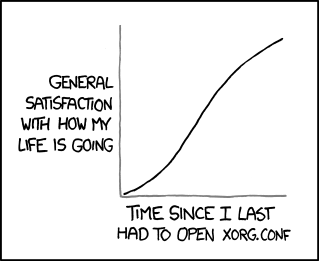
\includegraphics[width=0.80\paperwidth,height=0.80\textheight]{graphics/xkcd-x11-1.png}}
    \end{center}
\end{frame}

% -------------------------------------------------------------------

\end{document}
